%%%%%%%%%%%%%%%%%%%%%%%%%%%%%%%%%%%%%%%%%
% University/School Laboratory Report
% LaTeX Template
% Version 3.1 (25/3/14)
%
% This template has been downloaded from:
% http://www.LaTeXTemplates.com
%
% Original author:
% Linux and Unix Users Group at Virginia Tech Wiki 
% (https://vtluug.org/wiki/Example_LaTeX_chem_lab_report)
%
% License:
% CC BY-NC-SA 3.0 (http://creativecommons.org/licenses/by-nc-sa/3.0/)
%
%%%%%%%%%%%%%%%%%%%%%%%%%%%%%%%%%%%%%%%%%

%----------------------------------------------------------------------------------------
%	PACKAGES AND DOCUMENT CONFIGURATIONS
%----------------------------------------------------------------------------------------

\documentclass{ctexart}

\usepackage[version=3]{mhchem} % Package for chemical equation typesetting
\usepackage{siunitx} % Provides the \SI{}{} and \si{} command for typesetting SI units
\usepackage{graphicx} % Required for the inclusion of images
\usepackage{natbib} % Required to change bibliography style to APA
\usepackage{amsmath} % Required for some math elements 
%\usepackage{showframe} % for showing page frames


\setlength\parindent{0pt} % Removes all indentation from paragraphs

\renewcommand{\labelenumi}{\alph{enumi}.} % Make numbering in the enumerate environment by letter rather than number (e.g. section 6)

%\usepackage{times} % Uncomment to use the Times New Roman font

%==========pesusdo codes
\usepackage[linesnumbered,boxed]{algorithm2e}
%\renewcommand{\algorithmcfname}{算法}
\renewcommand{\repeat}{Repeat}

%==========citation===========
%\usepackage{cite}
\usepackage{url}


% ==========添加首行缩进,两个字符===========
\usepackage{indentfirst}
\setlength{\parindent}{2em}
% ==========强制图片位置===========
\usepackage{float}

% ==========特殊数学符号===========
\usepackage{mathtools}
\usepackage{dsfont}
\usepackage{amsfonts}
% ==========列表===========
\usepackage{enumerate}

%----------------------------------------------------------------------------------------
%	DOCUMENT INFORMATION
%----------------------------------------------------------------------------------------

\title{采样——MCMC} % Title

%\author{fengmi \textsc{Feng}} % Author name

\author{Mia Feng} % Author name

\date{\today} % Date for the report

\begin{document}

\maketitle % Insert the title, author and date

%\begin{center}
%\begin{tabular}{l r}
%Date Performed: & January 1, 2012 \\ % Date the experiment was performed
%Partners: & James Smith \\ % Partner names
%& Mary Smith \\
%Instructor: & Professor Smith % Instructor/supervisor
%\end{tabular}
%\end{center}

% If you wish to include an abstract, uncomment the lines below
% \begin{abstract}
% Abstract text
% \end{abstract}

%----------------------------------------------------------------------------------------
%	SECTION 1
%----------------------------------------------------------------------------------------

\section{概述}
MCMC:粗暴的采样模拟方式,用于模拟直接计算困难的分布。用于采样,数值积分等等。蒙特卡洛采样方法的一个重要好处是:估计值的精度与$x$的维度无关,而是与采样次数有关。实际问题中采样二十次左右就能达到较好的精度。
%To determine the atomic weight of magnesium via its reaction with oxygen and to study the stoichiometry of the reaction (as defined in \ref{definitions}):

求解目标:用多次采样得到的频率分布近似原概率分布。即本来对复杂的$f\left(x\right)$做积分,但是因为$f\left(x\right)$比较复杂所以显式积分困难。迂回方法是构造统计量$\frac{f\left(x\right)}{p\left(x\right)}$,通过对$x\sim p\left(x\right)$进行采样(后文叙述中的目标分布$\pi\left(x\right)$指的就是它),求取统计量$\frac{f\left(x\right)}{p\left(x\right)}$的期望得到数值积分值。
\begin{equation}
\theta = \int_{a}^{b}f\left(x\right)\,dx=\int_{a}^{b}\frac{f\left(x\right)}{p\left(x\right)}p\left(x\right)\,dx\approx \frac{1}{n}\sum\limits_{i=0}^{n-1}\frac{f\left(x_i\right)}{p\left(x_i\right)}
\end{equation}

求解思路:微积分思想(recall:学习微积分的时候,用无数个划分的小矩形的面积来近似面积,但是当时的小矩形是来自均匀分布的)。实际上,来自均匀分布的可能性很小,此时需要考虑对复杂分布如何模拟采样,一旦完成对复杂分布的描述就可以完成数值积分。

\begin{figure}[H]
\begin{center}
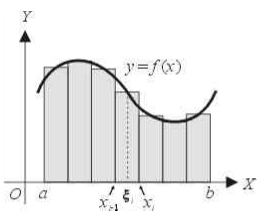
\includegraphics[width=0.8\textwidth]{fig/integration.png} % Include the image placeholder.png
\caption{矩形近似}
\end{center}
\end{figure}


求解方法:Markov Chain,蒙特卡洛积分,Metroplis-Hasting,Gibbs。

思维导图:详见MCMC.xmind
\begin{figure}[H]
\begin{center}
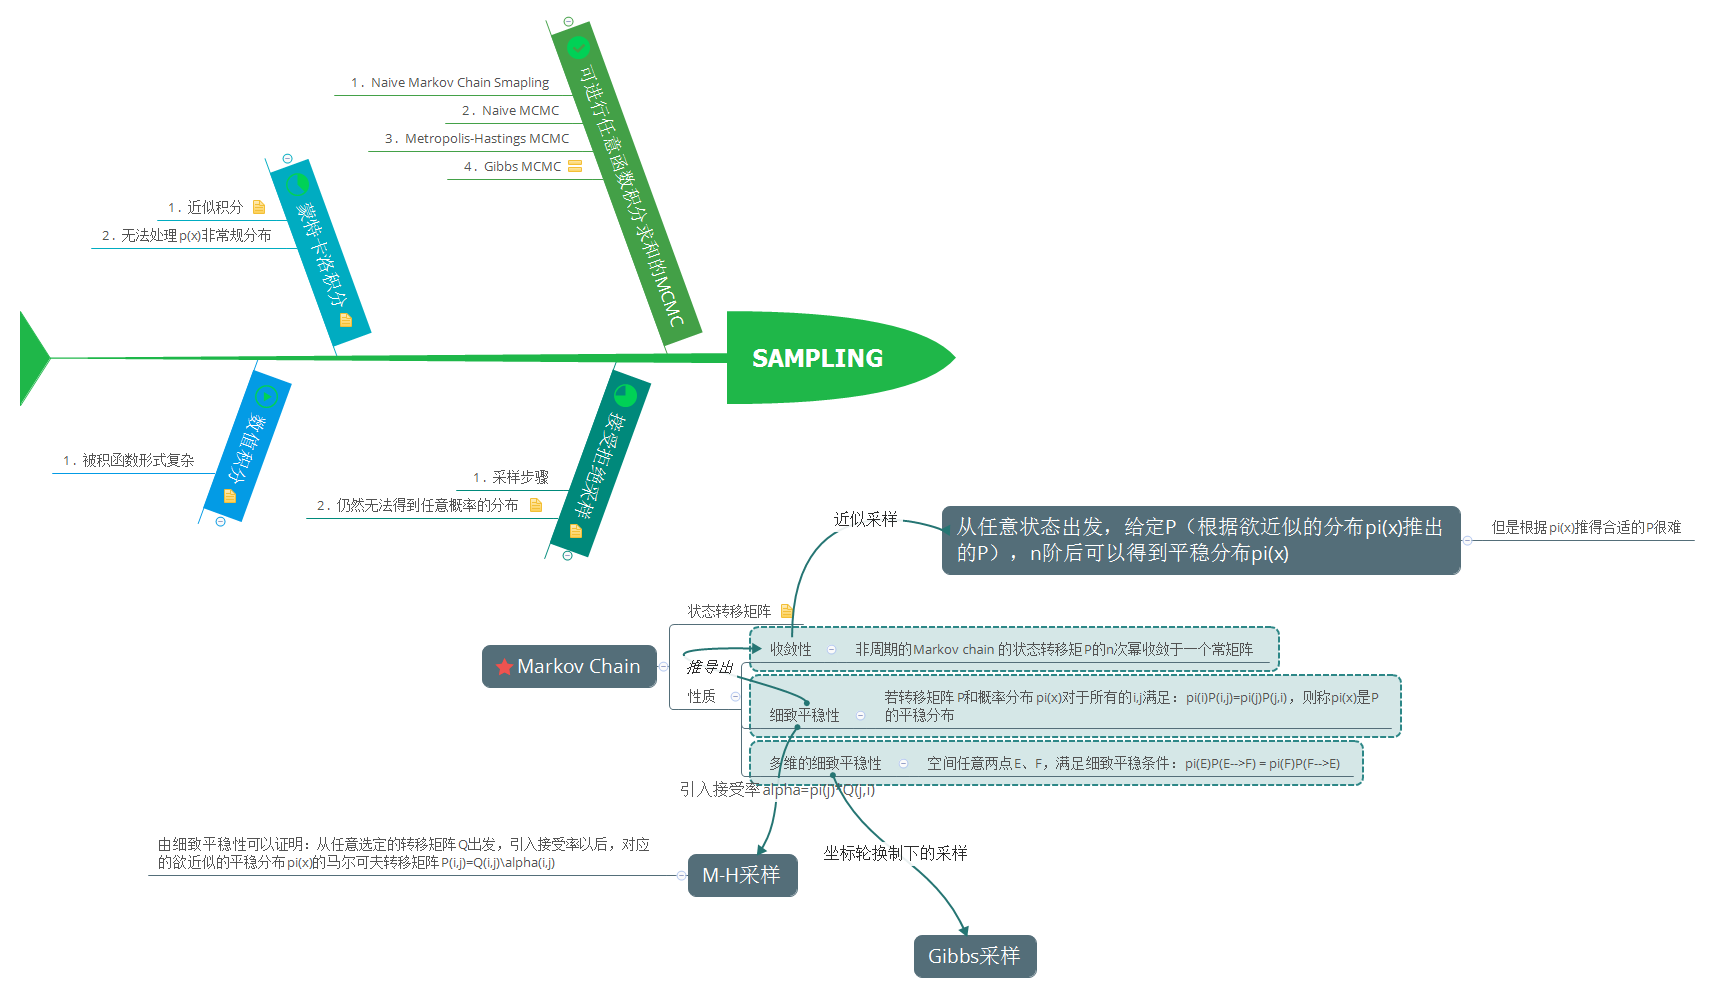
\includegraphics[width=0.8\textwidth]{fig/Sampling.png} % Include the image placeholder.png
\caption{思维导图}
\end{center}
\end{figure}


% If you have more than one objective, uncomment the below:
%\begin{description}
%\item[First Objective] \hfill \\
%Objective 1 text
%\item[Second Objective] \hfill \\
%Objective 2 text

\subsection{基础概念}
\label{distribution}
\begin{description}
\item[提议密度(Proposal Density)]
记提议密度为$q\left(x\right)$,其需要满足:
\begin{enumerate}[-]
\begin{item}
对$q\left(x\right)$ \emph{采样比较容易}。
\end{item}
\begin{item}
 $q\left(x\right)$的形状接近$\pi \left(x\right)$,具有
 \begin{equation}
 \pi \left(x\right) \le  Mq\left(x\right),\forall x
 \end{equation}
 其中$k$为常数。
\end{item}
\end{enumerate}

\end{description}

\subsection{马尔科夫链的性质}
\label{concepts}
\begin{description}
\item[马尔可夫矩阵的收敛性]
可以参考MIT的线性代数课程中对马尔可夫矩阵的讲述。马尔可夫矩阵中各元素大于0且小于1,而且矩阵是对称矩阵。马尔可夫矩阵的特征值中有一个为1,其余都是比1小的正数,所以马尔可夫矩阵的n次幂收敛至一个常数,这也是为什么马尔科夫链一定会收敛,最终可以模拟一个平稳分布的原因。而且,每个马尔科夫链对应的稳定分布是唯一的。(唯一性证明请自行百度,尚未查阅这方面的资料)

\item[马尔科夫链的细致平稳条件]
如果非周期马尔科夫链的状态转移矩阵$P$和概率分布$\pi\left(x\right)$对于所有的$i,j$满足
\begin{equation}
\pi\left(i\right)P\left(i,j\right)=\pi\left(j\right)P\left(j,i\right)
\end{equation}
则称概率分布$\pi\left(x\right)$是状态转移矩阵$P$的平稳分布。所以,利用对应的状态转移矩阵$P$,就可以模拟平稳复杂分布$\pi$。但是对于任意的平稳分布$\pi$,$P$的构造比较困难。MCMC采用迂回的方式解决了这个问题。

\item[多维数据的马尔可夫链的细致平稳条件]

平面上任意两点$E,F$,满足细致平稳条件
\begin{equation}
\pi\left(E\right)P\left(E\to F\right)=\pi\left(F\right)P\left(F\to E\right)
\end{equation}
取上一状态的条件概率分布即可作为马尔科夫链的状态转移概率。固定$n-1$维,只改变一维。这样按坐标轴轮换完成整个特征维的状态转移后,算完成一次。

\end{description}




\subsection{采样方法}
\label{sampling}
\begin{description}

\item[接受——拒绝采样]
可以参考Metropolis接受准则,核心思想是当能量增加时以一定概率接收,而不是一味的拒绝。

当公式$\left(1\right)$中的$p\left(x\right)$不是常见分布时,无法根据$p\left(x\right)$对$x$直接进行采样。此时接受——拒绝采样可以完成对$x$的模拟采样。

选定提议密度$q\left(x\right)$,如高斯分布、均匀分布等。先根据提议分布$q\left(x\right)$采样得到一个样本$x_0$,其对应的实际的概率是$u_0$。再从均匀分布$\left(0,kq\left(x_0\right)\right)$中采样得到一值$u$,若$u<u_0$,接受这次采样值$x_0$,反之拒绝。
步骤为:
\begin{enumerate}[-]
\begin{item}
产生样本$x_0\sim q\left(x\right)$以及$u  \sim Uniform\left(0,kq\left(x_0\right)\right)$。
\end{item}
\begin{item}
 若$u\le p\left(x_0\right)$,则接受$x_0$,反之拒绝。
\end{item}
\end{enumerate}


注:为与MCMC中的接受率叙述保持一致,这里对接受拒绝准则重述如下:


步骤为:
\begin{enumerate}[-]
\item
产生样本$x_0\sim q\left(x\right)$以及$u  \sim Uniform\left(0,1\right)$。

\item
 若$u\le \frac{p\left(x_0\right)}{kq\left(x_0\right)}$,则接受$x_0$,反之拒绝。

\end{enumerate}
其中,接受率$\alpha=\frac{p\left(x_0\right)}{kq\left(x_0\right)}$,是图3中红色曲线的面积与蓝色曲线的面积的比值。其理论值为
\begin{equation}
\alpha^* = \frac{\int_a^b p\left(x\right) \,dx}{k\int_a^b q\left(x\right) \,dx}=\frac{1}{k}
\end{equation}

当然,$k,q\left(x\right)$的选取要满足提议密度的性质:$kq\left(x\right)\ge p\left(x\right)$。但是满足这个条件比较困难,MCMC中Metropolis-Hastings方法将解决这个问题。

而且,高维空间的$k$将非常大,计算所得的接受率极小,相应的拒绝率会非常高,这导致了采样效率不高\cite{mcmc:Xu}。


\begin{figure}[H]
\begin{center}
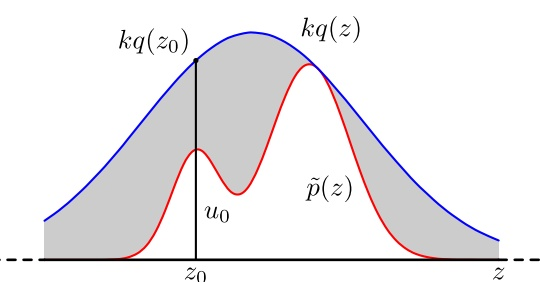
\includegraphics[width=0.8\textwidth]{fig/kq(x)--x.jpg} % Include the image placeholder.png
\caption{接受拒绝采样}
\end{center}
\end{figure}

\item[重要性采样]
为了提升简单接受——拒绝采样方法的采样效率。无需严格满足$p\left(x\right)\le kq\left(x\right)$。
\begin{equation}
\theta = \int_{a}^{b}f\left(x\right)\,dx=\int_{a}^{b}\frac{f\left(x\right)}{p\left(x\right)}\frac{p\left(x\right)} {q\left(x\right)}q\left(x\right)  \,dx
\end{equation}
重要性$w$记为:
\begin{equation}
w=\frac{p\left(x\right)} {q\left(x\right)}
\end{equation}
其余的定义不变。


则原数值积分值$\theta$的近似计算步骤为:
\begin{enumerate}[-]
\item
产生样本$x_1,\cdots, x_n \sim q\left(x\right)$。

\item
计算对积分值$\theta$的无偏估计为
\begin{equation}
\hat{I}=\frac{1}{n}\sum\limits_{i=1}^{n}\frac{f\left(x_i\right)}{p\left(x_i\right)}w\left(x_i\right)
\end{equation}
其中$w\left(x_i\right)=\frac{p\left(x_i\right)} {q\left(x_i\right)}$
实际中常用有偏估计来近似积分值$\theta$,公式为:
\begin{equation}
\hat{I}=\frac{\sum\limits_{i=1}^{n}\frac{f\left(x_i\right)}{p\left(x_i\right)}w\left(x_i\right)}{\sum\limits_{i=1}^{n}w\left(x_i\right)}
\end{equation}
\end{enumerate}
与接受——拒绝采样中类似,这里的提议密度$q\left(x\right)$也是任意的。只是当$q\left(x\right)$与$p\left(x\right)$更接近,并且 $q\left(x\right)$尾部较厚的时候方差更小(更近均匀分布),提议密度的采样效率更高。(这里\emph{不再需要满足}$p\left(x\right)\le kq\left(x\right)$) 。
当然,只有当$q\left(x\right)$与$p\left(x\right)$更接近时,$w\left(x\right)$的取值范围会更小一些,否则其取值范围还是很大,还是没法完成对任意分布的近似。


\item[马尔科夫链采样]
选定平稳分布$\pi \left(x\right)$的状态转移矩阵$P$之后,根据状态转移矩阵$P$,不断完成上一状态到下一状态的转移得到此时的条件概率,利用此时的条件概率得到采样值,重复这个转移过程直至条件概率收敛。收敛之后的采样集可以作为采样结果输出用于蒙特卡洛模拟求和。
设计不同的马尔科夫状态转移矩阵$P$(下文中记为$Q$),就得到了下述几种不同的采样方法。

\item[MCMC采样——Metropolis采样]
接受——拒绝原理是相同的,与MH采样方法不同在Metropolis的转移矩阵$Q$是对称矩阵,即由上一状态转移到当前状态和由当前状态转移到上一状态的概率是相等的。

通过比较采样自均匀分布$\left(0,1\right)$的值u与接受率$\alpha\left(i,j\right)$,决定是否接受转移。

因为采用马尔科夫链,这里的接受率定义为:
\begin{equation}
\alpha = \min\left(1,\frac{\pi\left(j\right)}{\pi\left(i\right)}\right)
\end{equation}

\begin{figure}[H]
\begin{center}
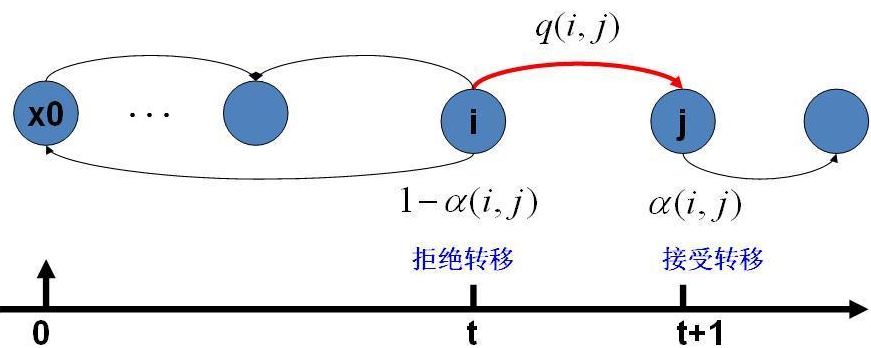
\includegraphics[width=0.8\textwidth]{fig/mc-trans.png} % Include the image placeholder.png
\caption{马氏链转移和接受概率}
\end{center}
\end{figure}



\item[MCMC采样——Metropolis-Hastings采样]
接受——拒绝原理是相同的,但是这里的提议分布是根据马尔科夫链状态转移后得到的。状态转移矩阵$Q$是非对称矩阵。Metropolis采样可以看做Metropolis-Hastings采样的一个特例。
接受率定义为:
\begin{equation}
\alpha = \min\left(1,\frac{\pi\left(j\right)Q\left(j,i\right)}{\pi\left(i\right)Q\left(i,j\right)}\right)
\end{equation}


\item[MCMC采样——Gibbs采样]
与马尔可夫随机场模型比较接近。\text{\color{red}{待补充}}。


\end{description}




%----------------------------------------------------------------------------------------
%	SECTION 2
%----------------------------------------------------------------------------------------

\section{算法实现}
%见CS229\cite{stanf:cs229}
%
%\begin{enumerate}[1.]
%\item 随机初始化cluster centroids $\mu_1,\mu_2,\cdots,\mu_k\in\mathbb{R}^n$
%\item 迭代直至收敛\{
%
%对于每一个样例$i$,计算类标
%\begin{equation}
%c^{\left(i\right)}\coloneqq \arg\min\limits_{j}\big\| x^{\left(i\right)}-\mu_{j}\big\|^2
%\end{equation}
%对于每一个类$j$,更新cluster centroids:
%\begin{equation}
%\mu_j \coloneqq \frac{\sum\limits_{i=1}^{m}\mathds{1}\left\{c^{\left(i\right)}=j\right\}x^{\left(i\right)}}{\sum\limits_{i=1}^{m}\mathds{1}\left\{c^{\left(i\right)}=j\right\}}
%\end{equation}
%\}
%\end{enumerate}
注意实现时取了拉普拉斯平滑,见公式$\big(4\big)$,且为了防止下溢取对概率值取了对数。\cite{mcmc:Liu}
%----------------------------------------------------------------------------------------
%	SECTION 3
%----------------------------------------------------------------------------------------
%
\section{Implementation}
%MCMC
%\begin{figure}[H]
%\begin{center}
%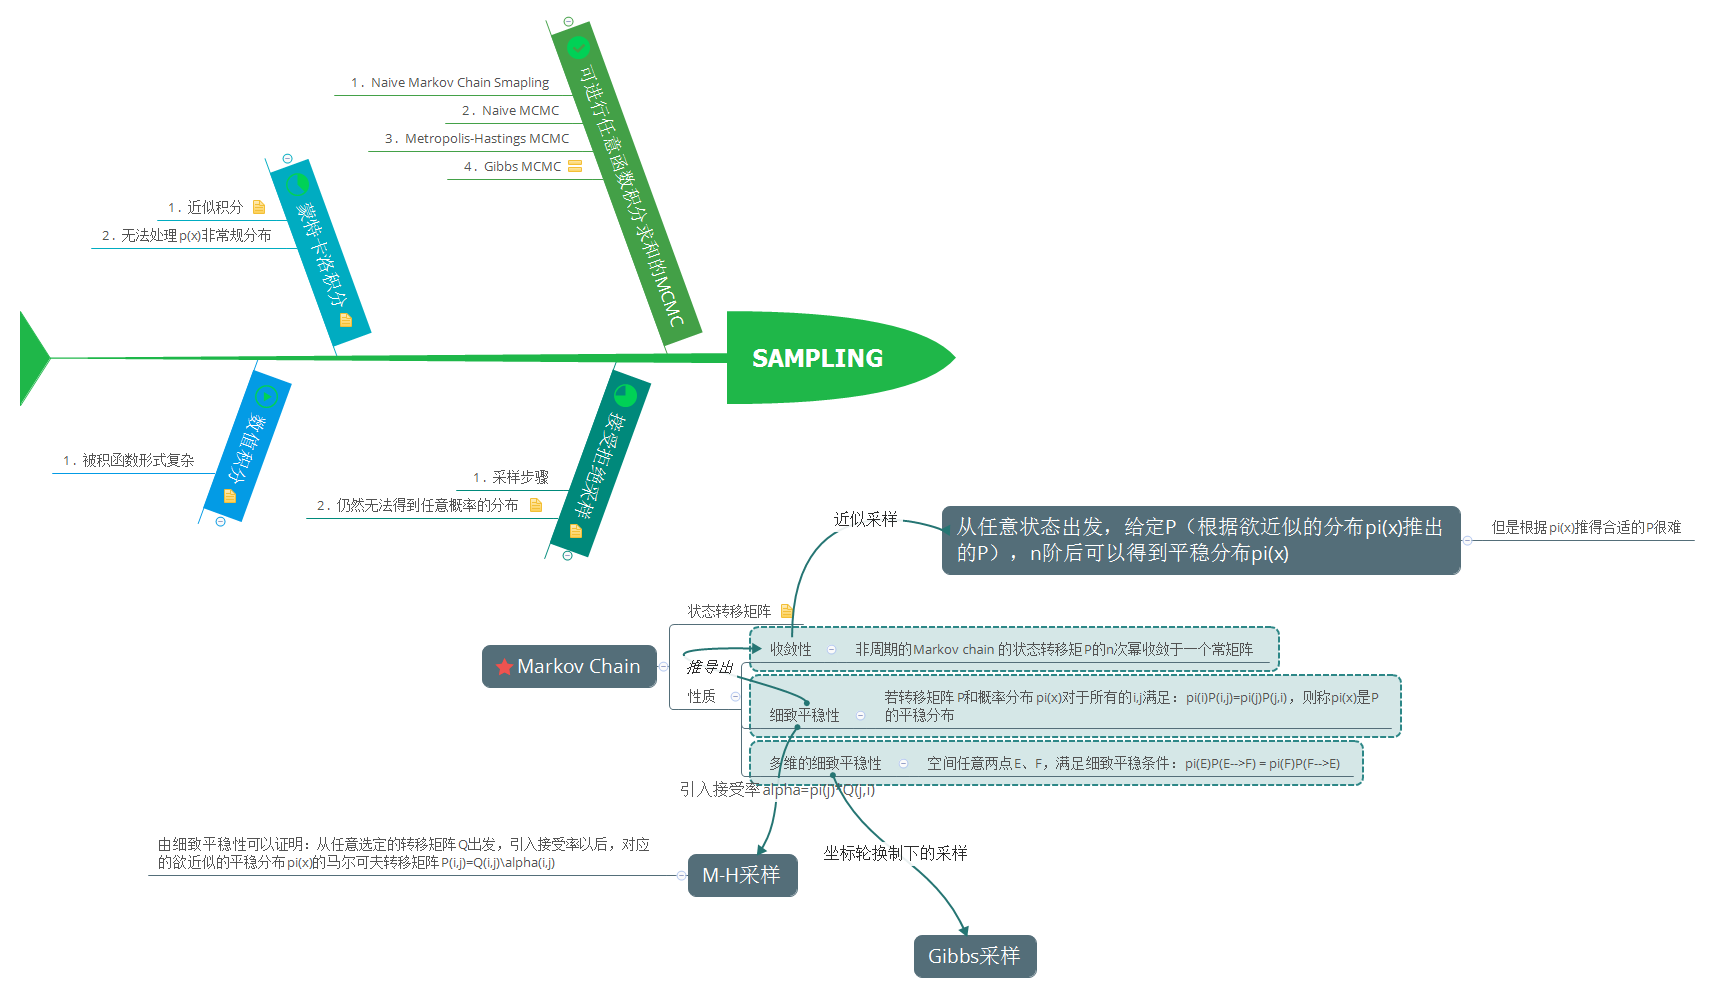
\includegraphics[width=0.8\textwidth]{fig/Sampling.png} % Include the image placeholder.png
%\caption{MCMC思维导图}
%\end{center}
%\end{figure}

%%----------------------------------------------------------------------------------------
%%	SECTION 4
%%----------------------------------------------------------------------------------------
%
%\section{Results and Conclusions}
%
%The atomic weight of magnesium is concluded to be \SI{24}{\gram\per\mol}, as determined by the stoichiometry of its chemical combination with oxygen. This result is in agreement with the accepted value.
%
%\begin{figure}[h]
%\begin{center}
%\includegraphics[width=0.65\textwidth]{placeholder} % Include the image placeholder.png
%\caption{Partial Gradient of $L_\big(\theta \big)$}
%\end{center}
%\end{figure}
%
%%----------------------------------------------------------------------------------------
%%	SECTION 5
%%----------------------------------------------------------------------------------------
%
%\section{Discussion of Experimental Uncertainty}
%
%The accepted value (periodic table) is \SI{24.3}{\gram\per\mole} \cite{Smith:2012qr}. The percentage discrepancy between the accepted value and the result obtained here is 1.3\%. Because only a single measurement was made, it is not possible to calculate an estimated standard deviation.
%
%The most obvious source of experimental uncertainty is the limited precision of the balance. Other potential sources of experimental uncertainty are: the reaction might not be complete; if not enough time was allowed for total oxidation, less than complete oxidation of the magnesium might have, in part, reacted with nitrogen in the air (incorrect reaction); the magnesium oxide might have absorbed water from the air, and thus weigh ``too much." Because the result obtained is close to the accepted value it is possible that some of these experimental uncertainties have fortuitously cancelled one another.
%
%%----------------------------------------------------------------------------------------
%%	SECTION 6
%%----------------------------------------------------------------------------------------
%
%\section{Answers to Definitions}
%
%\begin{enumerate}
%\begin{item}
%The \emph{atomic weight of an element} is the relative weight of one of its atoms compared to C-12 with a weight of 12.0000000$\ldots$, hydrogen with a weight of 1.008, to oxygen with a weight of 16.00. Atomic weight is also the average weight of all the atoms of that element as they occur in nature.
%\end{item}
%\begin{item}
%The \emph{units of atomic weight} are two-fold, with an identical numerical value. They are g/mole of atoms (or just g/mol) or amu/atom.
%\end{item}
%\begin{item}
%\emph{Percentage discrepancy} between an accepted (literature) value and an experimental value is
%\begin{equation*}
%\frac{\mathrm{experimental\;result} - \mathrm{accepted\;result}}{\mathrm{accepted\;result}}
%\end{equation*}
%\end{item}
%\end{enumerate}

%----------------------------------------------------------------------------------------
%	BIBLIOGRAPHY
%----------------------------------------------------------------------------------------
%
% 注意一定要在文中引用才不会出错(至少引用一个)
\bibliographystyle{plain}
\bibliography{bib//mcmc}

%----------------------------------------------------------------------------------------


\end{document}